\documentclass{beamer}

\usepackage{tikz}
\usetikzlibrary{shapes.multipart}

\usepackage[dvipsnames]{xcolor}

\usepackage{biblatex}
\bibliography{../../../references.bib}

%Information to be included in the title page:
\title{Understanding the Structure of District Heating Networks from Measurement Data}
\subtitle{A First Overview}
\author{Fabian Weik}
\institute{Fraunhofer ITWM}
\date{\today}

\begin{document}

\frame{\titlepage}

\begin{frame}
\frametitle{Motivation}
  \begin{itemize}
    \item Sometimes, the information about the structure of district heating networks is incomplete
    \item But needed for precise simulation
      \begin{itemize}
        \item Model does not have to be identical to real network
        \item Rather it should act similarly to the real network
      \end{itemize}
  \end{itemize}
\end{frame}

\begin{frame}
\frametitle{State of the Art Simulation}
  \begin{figure}
    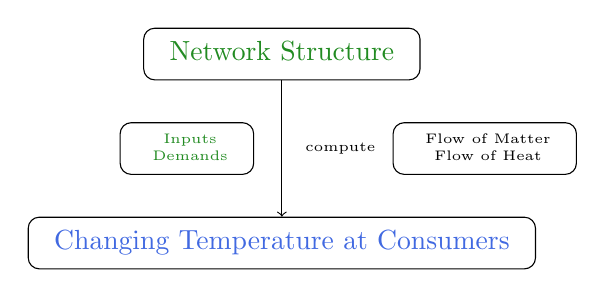
\begin{tikzpicture}
      \node (A) [rectangle, draw, rounded corners] at (0, 1.2) {
        \begin{tabular}{c}
          \color{ForestGreen}
          Network Structure
        \end{tabular}
      };
      \node (B) [rectangle, draw, rounded corners] at (0, -1.2) {
        \begin{tabular}{c}
          \color{RoyalBlue}
          Changing Temperature at Consumers
        \end{tabular}
      };

      \draw[->] (A) to (B) node [midway, right, xshift=5] {\tiny{compute}}
        node [midway, right, rectangle, draw, rounded corners, xshift=40] {\tiny{
          \begin{tabular}{c}
            Flow of Matter \\
            Flow of Heat
          \end{tabular}
        }}
        node [midway, left, rectangle, draw, rounded corners, xshift=-10] {\tiny{
          \begin{tabular}{c}
            \color{ForestGreen}
            Inputs \\
            \color{ForestGreen}
            Demands \\
          \end{tabular}
        }};
    \end{tikzpicture}
  \end{figure}
\end{frame}

\begin{frame}
\frametitle{Identifying the Structure --- Goal}
  \begin{figure}
    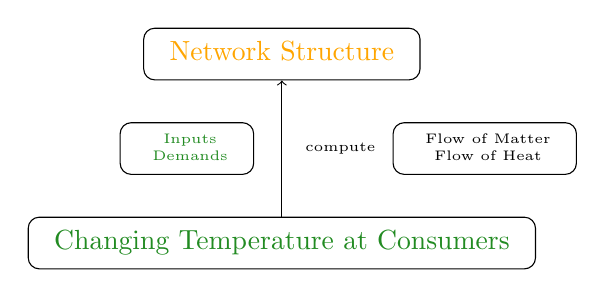
\begin{tikzpicture}
      \node (A) [rectangle, draw, rounded corners] at (0, 1.2) {
        \begin{tabular}{c}
          \color{Orange}
          Network Structure
        \end{tabular}
      };
      \node (B) [rectangle, draw, rounded corners] at (0, -1.2) {
        \begin{tabular}{c}
          \color{ForestGreen}
          Changing Temperature at Consumers
        \end{tabular}
      };

      \draw[<-] (A) to (B) node [midway, right, xshift=5] {\tiny{compute}}
        node [midway, right, rectangle, draw, rounded corners, xshift=40] {\tiny{
          \begin{tabular}{c}
            Flow of Matter \\
            Flow of Heat
          \end{tabular}
        }}
        node [midway, left, rectangle, draw, rounded corners, xshift=-10] {\tiny{
          \begin{tabular}{c}
            \color{ForestGreen}
            Inputs \\
            \color{ForestGreen}
            Demands \\
          \end{tabular}
        }};
    \end{tikzpicture}
  \end{figure}

  \vspace{1em}

  Somehow compute in the other direction
\end{frame}

\begin{frame}
\frametitle{Simulation Details}
  Can be split into two parts

  \vspace{1em}

  \begin{itemize}
    \item Hydraulic (computes mass flux)
      \begin{itemize}
        \item Non-linear
        \item Requires computing loops in the network
      \end{itemize}
    \item Thermal (computes heat based on mass flux)
      \begin{itemize}
        \item Basically linear
        \item Influences the hydraulic problem in the next step
      \end{itemize}
  \end{itemize}
\end{frame}

\begin{frame}
\frametitle{Identifying the Structure --- Approach I}
  Formulate finding the structure as a optimization problem.

  \vspace{2em}

  \begin{itemize}
    \item Possible Connections as parameters
      \begin{itemize}
        \item Single values of edge icidence matrix
        \item Influences loop incidence matrix also
      \end{itemize}
    \item Optimize for low error (discrepancy to measured data)
  \end{itemize}

  \vspace{2em}

  Possibly
  \begin{itemize}
    \item Connections as continuous values instead of discrete
  \end{itemize}
\end{frame}

\begin{frame}
\frametitle{Approach I --- Possible Optimizations}
  \begin{itemize}
    \item Use already computed loops to speed up computation of the loops in the new structure
    \item Reducing the problem space:
    \begin{itemize}
      \item Only check connections that make sense
        \begin{itemize}
          \item Based on coordinates
          \item Based on streets
        \end{itemize}
      \item Use heuristics to check most likely first
    \end{itemize}
    \item Compute a initial guess with a linear heat/mass transfer model (based on~\cite{wang2024identification})
  \end{itemize}
\end{frame}

\begin{frame}
\frametitle{Identifying the Structure --- Approach II}
  \begin{itemize}
    \item Calculate possible connections and mass flux
    \item Check whether mass flux is possible with supply and demand
    \begin{itemize}
      \item Solution to the hydraulic problem?
    \end{itemize}
  \end{itemize}

  \begin{figure}
    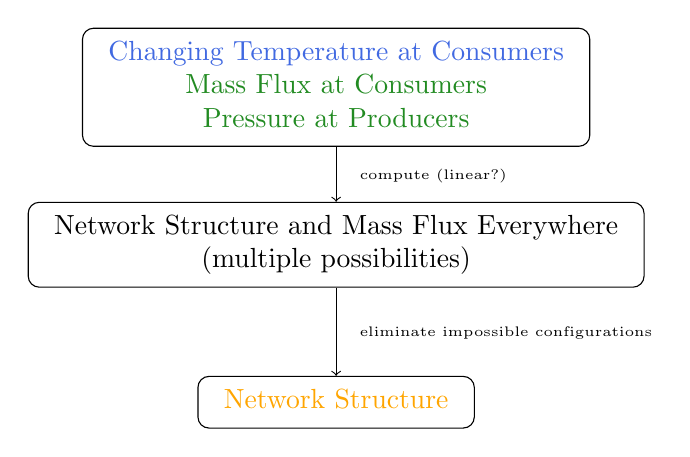
\begin{tikzpicture}
      \node (A) [rectangle, draw, rounded corners] at (0, 2.0) {
        \begin{tabular}{c}
          \color{RoyalBlue} Changing Temperature at Consumers \\
          \color{ForestGreen} Mass Flux at Consumers \\
          \color{ForestGreen} Pressure at Producers
        \end{tabular}
      };
      \node (B) [rectangle, draw, rounded corners] at (0, 0) {
        \begin{tabular}{c}
          Network Structure and Mass Flux Everywhere \\
          (multiple possibilities)
        \end{tabular}
      };
      \node (C) [rectangle, draw, rounded corners] at (0, -2.0) {
        \begin{tabular}{c}
          \color{Orange} Network Structure
        \end{tabular}
      };

      \draw[->] (A) to (B) node [midway, right, xshift=5, yshift=25] {\tiny{compute (linear?)}};
      \draw[->] (B) to (C) node [midway, right, xshift=5, yshift=-32] {\tiny{eliminate impossible configurations}};
    \end{tikzpicture}
  \end{figure}
\end{frame}

%\begin{frame}
%\frametitle{Approach II --- Challenges}
%  \begin{itemize}
%    \item The change in flow (Vorlauf) temperature at the consumers leads to a change in velocity at the consumers, assuming constant power demand
%    \begin{itemize}
%      \item Introduces discontinuities because of possibly changing directions of mass flux
%      \item Makes the problem non-linear
%    \end{itemize}
%  \end{itemize}
%\end{frame}

\begin{frame}
\frametitle{Measurements and Signals}
  Measurements:
  \begin{itemize}
    \item Temperature and pressure at the producers
    \item Temperature and mass flux at consumers
  \end{itemize}

  \vspace{2em}

  Signals:
  \begin{itemize}
    \item Temperature and pressure at the produers
    \item Possibly: mass flux at consumers (by reducing/increasing power)
  \end{itemize}
\end{frame}

\begin{frame}
\frametitle{Challenges}
  \begin{itemize}
    \item Some nodes might be unknown
      \begin{itemize}
        \item Can this be ignored, since we only care about the simulation results?
      \end{itemize}
    \item Temperatures and mass flux are only known at nodes adjacent to consumers
    \item Mass flux demand at consumers decreases when temperature increases
      \begin{itemize}
        \item Depend heavily on first increase of measured temperature
        \item Extract useful information from that timing
      \end{itemize}
  \end{itemize}
\end{frame}

\begin{frame}
\frametitle{To be Determined --- Loose Ideas}
  \begin{itemize}
    \item Useful signals to send into the network for most helpful data
      \begin{itemize}
        \item Pulse of temperature at producer
        \item Possibly: increse/decrease flow at a consumer
      \end{itemize}
    \item Possibility of optimizing connections continuously
    \item Possibilities of reducing problem space in case of discrete optimizations
      \vspace{1em}
    \item What other already techniques for identifying the structure of (electrical) networks may apply
  \end{itemize}
\end{frame}

\begin{frame}
\frametitle{References}
  \printbibliography
\end{frame}
\end{document}
